\section{Dynamische Analyse}
Die dynamische Analyse gewinnt, im Gegensatz zur statischen Analyse, über die Ausführung der Malware weitere Informationen. So können Verhaltensmuster, welche in der statischen Analyse nur grob vorherzusehen sind, beobachtet und weiter analysiert werden. Im Folgenden werden verschiedene Möglichkeiten und Tools zur dynamischen Analyse vorgestellt.

\subsection{Malwr}
Als erster Punkt der statischen Analyse wird die Datei \textit{f113} auf der Seite \textit{Malwr} (siehe Abschnitt \ref{ref:ToolsMalwr}) analysiert.

Dabei weist \textit{Malwr} auf folgende Eigenheiten hin:
\begin{itemize}
\item File has been identified by at least one AntiVirus on VirusTotal as malicious
\item The binary likely contains encrypted or compressed data.
\item Tries to unhook Windows functions monitored by Cuckoo
\item Executed a process and injected code into it, probably while unpacking
\end{itemize}
Demnach enthält die Datei verschlüsselte Daten, versucht aktiv Sandboxen zu vermeiden und lädt "on-the-fly" Code nach. Dies erklärt, warum die Analyse bisher und im weiteren Verlauf nicht vollständig durchlaufen werden kann. Dem vollständigen Report\footnote{\url{https://malwr.com/analysis/MDIwOTgyODFmOTFiNDU1NDk3ZWFiMzc1NzAwYWI2MGU/}} können weitere Daten entnommen werden.
Aus den gleichen Gründen wie bei \textit{Virustotal}, siehe \ref{ref:statAnVirustotal}, wird nun jedoch ein Großteil der Informationen lokal gesammelt.

\subsection{Live-Analyse}
Als Nächstes folgt die lokale Live-Analyse. Dazu sollte zuallererst ein Snapshot der Virtuellen Maschine erstellt werden, damit man die Maschine nach der Ausführung und Analyse wieder auf einen nicht-kompromittierten Zustand zurücksetzen kann. Im Anschluss werden vor der Analyse folgende Programme gestartet:
\begin{itemize}
	\item RegShot
	\item Process Monitor
	\item Wireshark
	\item Process Explorer
\end{itemize}
Nachdem alle Programme gestartet sind und aufzeichnen, kann die Malware (Datei \textit{f113}) ausgeführt werden. Im Folgenden sind die Ergebnisse aufgezeigt.

\subsubsection{Grundlegende Beobachtungen}
Nach der Ausführung des Programms öffnet sich kein Fenster. Dafür wird die Datei \textit{f113} im ursprünglichen Ordner gelöscht. Es kann keine weitere Aktion beobachtet werden.

\subsubsection{RegShot}
\label{ref:DynAnRegShot}
\textit{RegShot} liefert folgendes Log (gekürzt):
\begin{lstlisting}
Keys added:9 
HKU\S-1-5-21-12[..]00\Software\Microsoft\Multimedia\Audio
HKU\S-1-5-21-12[..]00\Software\Microsoft\Multimedia\Audio\Box
HKU\S-1-5-21-12[..]00\Software\Microsoft\Multimedia\Audio\Box\ba8c80406
HKU\S-1-5-21-12[..]00\Software\Microsoft\Multimedia\Audio\Box\ba8c80407
HKU\S-1-5-21-12[..]00\Software\Microsoft\Multimedia\Audio\Box\ba8c80408
HKU\S-1-5-21-12[..]00\Software\Rocal AppWizard-Generated Applications
HKU\S-1-5-21-12[..]00\Software\Rocal AppWizard-Generated Applications\BG
HKU\S-1-5-21-12[..]00\Software\Rocal AppWizard-Generated Applications\BG\Recent File List
HKU\S-1-5-21-12[..]00\Software\Rocal AppWizard-Generated Applications\BG\Settings
 

Values added:3 
HKU\S-1-5-21-12[..]00\Software\Microsoft\Windows\CurrentVersion\Explorer\UserAssist\{CE[..]EA}\Count\P:\Znyjner\81[..]86\s1[..]32.rkr:
	00 00 00 00 01 00 00 00 00 00 00 00 00 00 00 00 00 00 80 BF 
	00 00 80 BF 00 00 80 BF 00 00 80 BF 00 00 80 BF 00 00 80 BF
	00 00 80 BF 00 00 80 BF 00 00 80 BF 00 00 80 BF FF FF FF FF 
	00 88 32 0C E9 BE D0 01	00 00 00 00
HKU\S-1-5-21-12[..]00\Software\Microsoft\Windows\CurrentVersion\Internet Settings\GlobalUserOffline: 0x00000000
HKU\S-1-5-21-12[..]00\Software\Microsoft\Windows\CurrentVersion\Run\msdb2484d4d.exe: ""C:\Users\Dominik\AppData\Roaming\Microsoft\msdb2484d4d.exe""
\end{lstlisting}

Besonders interessant ist dabei der letzte Eintrag, welcher verrät, dass unter \\ \textit{C:\textbackslash Users\textbackslash Dominik\textbackslash AppData\textbackslash Roaming\textbackslash Microsoft\textbackslash msdb2484d4d.exe} ein neues Programm angelegt wurde, welches beim nächsten Start ausgeführt wird. Prüft man den Hash der Datei, entspricht dieser der Datei \textit{f113}, \textit{f113cf383214f2788876d27d644ab432}. Daher wird die Datei im Folgenden \textit{msdb} genannt. Diese wird unter dem oben genannten Pfad gehalten, um das Verhalten der Malware nicht negativ zu beeinflussen. Ebenfalls fallen die Einträge, welche "`Rocal AppWizard-Generated Applications"' enthalten, auf. Dieser String wurde bereits in der statischen Analyse mit Hilfe von \textit{PEView} unter Abschnitt \ref{ref:statAnPEView} gefunden.

\subsubsection{Process Monitor}
Aus dem \textit{Process Monitor}-Log konnten keine weiteren Kenntnisse gewonnen werden. Das Log ist (gefiltern nach der Datei \textit{f113}) unter \textit{f113cf383214f2788876d27d644ab432.CSV} an die Arbeit angehängt. Es konnte jedoch bestätigt werden, dass die Datei \textit{msdb} geschrieben und zum Autostart hinzugefügt wurde (siehe Abbildung \ref{img:ProcMonf113}). Die Datei \textit{msdb} scheint nicht direkt aufgerufen worden zu sein. Zumindest zeigt der Filter keinen Treffer für \textit{msdb}.

\begin{figure}[htbp]
	\centering
	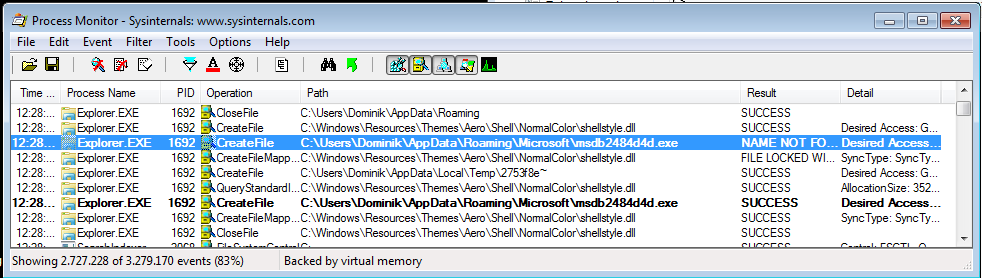
\includegraphics[width=\textwidth]{bilder/dynamischeAnalyse/ProcessMonitor.png}
	\caption{Process Monitor nach Ausführung von \textit{f113} zeigt die Erstellung von \textit{msdb}}
	\label{img:ProcMonf113}
\end{figure}

\subsubsection{Wireshark}
Es konnte kein von der Malware in diesem Stadium ausgelöster Netzwerkverkehr festgestellt werden.

\subsubsection{Process Explorer}
Im \textit{Process Explorer} können Post-Mortem keine Anomalien festgestellt werden. Über das Aufrufen von \textit{Optionen} $\rightarrow$ \textit{Virus Total} $\rightarrow$ \textit{Check Virustotal} können die Hashes aller aktuell laufenden Prozesse gegen die Onlinedatenbank geprüft werden. Dabei wurden alle Prozesse negativ getestet (siehe Abbildung \ref{img:ProcExpf113}). Daraus lässt sich vermuten, dass die Malware zumindest nach der ersten direkten Ausführung nicht mehr läuft. Nachdem die Datei \textit{msdb} jedoch bei einem Neustart des Rechners ausgeführt wird, könnten sich nach einem Neustart neue Funktionen zeigen.

\subsubsection{Autoruns}
Über das Tool \textit{Autoruns} kann die Erkenntnis aus \ref{ref:DynAnRegShot} verifizert werden. Wie unter der Abbildung \ref{img:Autorunsf113} zu sehen ist, wurde ein Autostart-Eintrag für die Datei \textit{msdb} erstellt.

\begin{figure}[htbp]
	\centering
	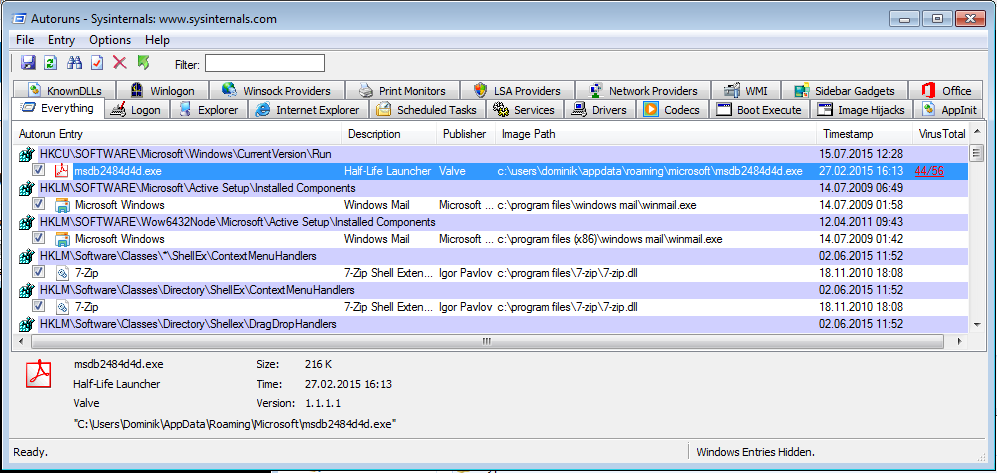
\includegraphics[width=\textwidth]{bilder/dynamischeAnalyse/autoruns.png}
	\caption{\textit{Autoruns} nach Ausführung von \textit{f113}}
	\label{img:Autorunsf113}
\end{figure}

\subsection{Immunity Debugger}
\label{ref:dynAnImmunityDebug}
Nach der Analyse wird die Maschine auf den Zustand vor der Live-Analyse zurückgesetzt. Anschließend wird die Datei \textit{f113} mit dem \textit{Immunity Debugger} (siehe Beschreibung \ref{ref:ToolsImmunityDebugger}) untersucht. Dazu öffnet man das Tool und anschließend die Datei \textit{f113}. Das Fenster ist im Anhang in Abbildung \ref{img:ImmunityDebf113} dargestellt. Anschließend wird über die Tasten \textit{F7} (\textit{Step Into}) und \textit{F8} (\textit{Step Over}) die Ausführung gesteuert. Dabei sind vor allem System-Calls interessant, da diese meist ohne großen Aufwand auf Aktivitäten der Malware schließen lassen.\\[1ex]

Schon zu Beginn lassen sich Parallelen zwischen der Disassemblierung von \textit{IDA} und der Ausführung im Debugger herstellen. Dies ist im Anhang in Abbildung \ref{img:IDAtoImmunityf113} verdeutlicht.\\[1ex]

Später in der Laufzeit kommt man zu der in der statischen Analyse beschriebenen Entscheidung, ob die Unterfunktion \textit{sub\_402718} oder die Start-Funktion weiter ausgeführt werden soll. Die Situation kurz vor dem Vergleich ist im Anhang in der Abbildung \ref{img:IDAtoImmunity2f113} dargestellt. Da \textit{EBX} und \textit{ESI} nicht gleich sind, wird die \textit{Zero}-Flag nicht gesetzt und der Jump (\textit{jnz}) wird normalerweise ausgeführt. Damit würde das Programm in Unterfunktion fortfahren. Das folgende Verhalten gleicht dem bisher beschriebene Verhalten. Um zu testen, was passiert, wenn der Vergleich anders ausgeht, wird der Sprung \textit{JNZ} auf \textit{JE} manipuliert (welcher das Gegenstück zu \textit{JNZ} ist). Abbildung \ref{img:ImmunityDebJZf113} zeigt den Assemblercode nach der Anpassung.

\begin{figure}[htbp]
	\centering
	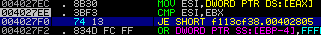
\includegraphics[width=\textwidth]{bilder/dynamischeAnalyse/ImmunityDebug2.png}
	\caption{Veränderung \textit{JNZ} zu \textit{JZ} während der Ausführung von \textit{f113}}
	\label{img:ImmunityDebJZf113}
\end{figure}

Leider führt diese weitere Ausführung auf eine \textit{Access-Violation}. Da Programme gezielt gegen Debugging geschützt werden können und eine solche Methode hier vermutlich zum Einsatz kommt, wurde die weitere Ausführung aufgegeben.

\subsection{Weiter Analyse}
Um das weitere Verhalten der Datei \textit{msdb} zu analysieren, wurden \textit{Process Monitor} und \textit{Wireshark} herangezogen. Zur Analyse der Datei \textit{msdb} bei einem Neustart wird im \textit{Process Monitor} die \textit{Option} $\Rightarrow$ \textit{Enable Boot Logging} aktiviert. Nach einem Neustart kann man nun die während der Bootzeit ausgeführten Aktionen analysieren.\\[1ex]

Wireshark zeigt wiederum keinen auffälligen Netzwerkverkehr. Das Log des \textit{Process Monitor} (welches nach dem Öffnen der Software nach dem Neustart angeboten wird) zeigt zwar, dass die Datei \textit{msdb} geladen wurde, zeigt aber keine weiteren Aktionen. Im \textit{Prozess Explorer} kann die Datei \textit{msdb} ebenfalls nicht als laufendes Programm gefunden werden.

\newpage
\subsection{Fazit zur dynamischen Analyse}
\label{ref:dynAnFazit}
Die dynamische Analyse konnte einige grundlegende Verhalten der Malware in Erfahrung bringen:
\begin{itemize}
	\item Die Ursprungs-Datei \textit{f113} löscht sich nach der Ausführung selbst.
	\item Die Datei \textit{msdb} wird nach der Ausführung von Datei \textit{f113} in den Ordner \\\textit{C:\textbackslash Users\textbackslash Dominik\textbackslash AppData\textbackslash Roaming\textbackslash Microsoft} kopiert.
	\item Für die Datei \textit{msdb} wird ein Autostart-Eintrag unter Software \\
\textit{\textbackslash Microsoft\textbackslash Windows\textbackslash CurrentVersion\textbackslash Run} angelegt
\end{itemize}
Leider konnten, vermutlich aufgrund der Eigenschaft, dass die Malware erkennt, dass sie analysiert wird, nicht alle Funktionalitäten in Erfahrung gebracht werden.